%! suppress = Makeatletter
%! suppress = Makeatletter
\documentclass[11pt]{report}

\usepackage[T1]{fontenc}
\usepackage[utf8]{inputenc}
\usepackage{graphicx}
\usepackage{amsmath,amssymb,amsfonts}
\usepackage{polski}
\usepackage[raggedright]{titlesec}
\usepackage{indentfirst}
\usepackage{listings}
\usepackage{hyperref}
\usepackage[backend=biber, bibencoding=utf8, style=ieee, dashed=false, isbn=false, doi=false, sorting=anyvt]{biblatex}
\usepackage{caption}
\captionsetup{%
justification=raggedright,
labelfont=bf,
singlelinecheck=off
}

\addbibresource{main.bib}

\pagestyle{headings}

\renewcommand{\chaptername}{Rozdział}
\renewcommand{\contentsname}{Spis treści}
\renewcommand{\figurename}{Rys.}
\renewcommand{\tablename}{Tab.}
\renewcommand{\listfigurename}{Spis rysunków}
\renewcommand{\listtablename}{Spis tabel}
\renewcommand{\bibname}{Bibliografia}

\makeatletter
\renewcommand{\l@section}{\@dottedtocline{1}{1.5em}{2.6em}}
\renewcommand{\l@subsection}{\@dottedtocline{2}{4.0em}{3.6em}}
\renewcommand{\l@subsubsection}{\@dottedtocline{3}{7.4em}{4.5em}}
\makeatother

\begin{document}
    \begin{titlepage}
        \centering
        \center{\scshape Sieciowe Systemy Multimedialne}
        \vspace{0.05\textheight}
        \center{\textbf CYFROWE ORGANY}
        \vspace{0.06\textheight}
        \center{\LARGE\bfseries Wykorzystanie symulatora wirtualnych organów piszczałkowych w celu poprawy brzmienia istniejącego instrumentu cyfrowego}
        \center{Using a virtual pipe organ simulator to improve the sound of an existing digital instrument}
        \vspace{0.5\textheight}
        \center{Michał Patyk}
        \vspace{0.03\textheight}
        \center{Kraków 2021}
    \end{titlepage}

    \tableofcontents


    \chapter{Wstęp}\label{ch:wstęp}
    Motywacją do wykonania projektu jest chęć poprawy brzmienia oraz zwiększenia możliwości istniejącego instrumentu cyfrowego.


    \chapter{Przegląd dziedziny}


    \section{MIDI}
    Musical Instrument Digital Interface (cyfrowy interfejs instrumentów muzycznych) to system służący do przekazywania informacji pomiędzy elektronicznymi instrumentami muzycznymi.
    Składa się z protokołu komunikacyjnego i specyfikacji sprzętowej.
    Powstał na początku lat osiemdziesiątych.
    W przeciwieństwie do strumieni audio, MIDI przekazuje cyfrową reprezentację wykonania, a nie właściwy dźwięk.

    Jak podaje~\cite{122929520160101}, są trzy typy portów MIDI: IN, OUT i THRU.
    Serializowane dane przesyłane są w kablu w jednym kierunku.
    MIDI OUT to wyjście danych do innego urządzenia.
    MIDI IN to wejście danych z innego urządzenia.
    MIDI THRU przekazuje wszystkie wiadomości które dotrą do urządzenia na port MIDI IN.

    Wiadomości MIDI sa podzielone na dwie kategorie: wiadomości systemowe i wiadomości kanałów.
    Wiadomości systemowe to te które sa związane z całym systemem MIDI.
    W każdej wiadomości kanałowej może być zakodowane do 16 kanałów, co pozwala na przesłanie jednym kablem wykonania składającego się z 16 różnych źródeł dźwięku.

    \section{Organy piszczałkowe}
    Organy piszczałkowe~\cite{329316420170801}, to jeden z najstarszych, wciąż często wykorzystywanych, instrumentów.
    Jednocześnie jest to największy i najbardziej złożony instrument.
    Najprostsze organy składają się z pojedynczego zestawu piszczałek, klawiatury (zwanej manuałem) w której każdy klawisz uwalnia powietrze do odpowiedniej piszczałki oraz urządzenia wytwarzającego ciśnienie powietrza.
    Bardziej złożone organy mają wiele rejestrów (zestawów piszczałek), kilka manuałów oraz pedał (klawiaturę nożną).
    Piszczałki mogą być skonstruowane z metalu lub drewna.
    Ich długość zaczyna się od kilku centymetrów, a może dochodzić do nawet 32 stóp (prawie 10 metrów).


    \section{Organy cyfrowe}
    Organy cyfrowe posiadają rozmaitą paletę głosów.
    Odwzorowanie brzmienia organów piszczałkowych tworzone jest najczęściej poprzez syntezę addytywną.
    W takim rodzaju syntezy przebiegi fal dźwiękowych nie są zapisywane bezpośrednio.
    Zamiast tego przechowywane są listy liczb określające amplitudy każdej harmonicznej,
    które są następnie wykorzystywane do tworzenia dźwięków w czasie rzeczywistym, zgodnie z wymaganiami.
    Kontuar (stół gry) organów cyfrowych zwykle wyglądem bardzo przypomina ten z organów piszczałkowych.
    Zgodnie z instrukcją Konferencji Episkopatu Polski organy elektroniczne wolno stosować tylko jako instrument tymczasowy,
    bez dodawania sztucznego prospektu (frontowej elewacji zewnętrznej).


    \section{Wirtualne organy piszczałkowe}

    \begin{figure}[!htp]
        \centering
        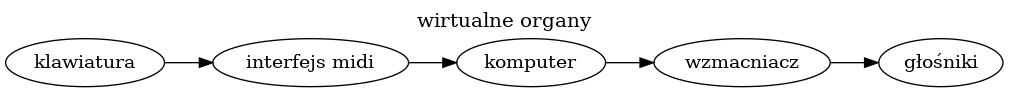
\includegraphics[width=\linewidth]{fig/organizacja.png}
        \caption{Schemat wykorzystania wirtualnych organów. (źródło:~opracowanie własne)}
        \label{fig:schemat}
    \end{figure}

    Komputer z odpowiednim oprogramowaniem może stać się symulatorem organów piszczałkowych.
    Dzięki wykorzystaniu próbek dokładnie odtwarza on brzmienie każdej piszczałki.
    Słyszalne są wszystkie szumy, stuki mechanizmu, do tego stopnia, że jest wręcz nie do odróżnienia, czy to grają wirtualne organy, czy też historyczny instrument.
    Próbki dźwięków zarejestrowane za pomocą mikrofonów zostają przypisane konkretnym klawiszom i pedałom.
    Rysunek~\ref{fig:schemat} przedstawia schemat wykorzystania typowych wirtualnych organów.


    \subsection{Sampling}
    Sampling to technika nagrywania dźwięków instrumentu muzycznego.
    Najprostsze rozwiązania to takie w których nagrywa się tylko kilka dźwięków, podczas gdy pozostałe są tworzone przez transponowanie.
    Najlepsze zestawy próbek to te w których każdy dźwięk jest nagrywany osobno.
    Niestety takie rozwiązanie, poza pracochłonnością procesu nagrywania, niesie też ze sobą problemy natury technicznej.
    Dźwięki powinny być przechowywane w najlepszym możliwie formacie, przy jak najwyższej częstotliwości próbkowania oraz wielobitowej kwantyzacji.
    W rezultacie powstaje duża ilość danych (kilka - kilkanaście gigabajtów).
    Dla najlepszej wierności dźwięku stosuje się tak zwane próbkowanie multi-release,
    w którym dla każdej piszczałki nagrywa się próbki rozpoczęcia, podtrzymania oraz wiele próbek zanikanie dźwięku.
    Taki zabieg wynika z faktu, że dźwięk zanikania ma inny charakter w zależności od długości nuty.
    Związane jest to z akustyką kościołów i hal koncertowych.
    Poza dźwiękami piszczałek, dla dodania realizmu, dołącza się też dźwięki mechanizmów, a nawet dmuchaw.


    \subsection{Oprogramowanie}

    Na rynku wirtualnych organów piszczałkowych istnieją dwaj duzi gracze: Hauptwerk oraz GrandOrgue.

    \paragraph{Hauptwerk}
    Hauptwerk to komercyjny program komputerowy stworzony w 2002 roku przez Martina Dyde'a~\cite{13115512220180101}, wydawany przez Milan Digital Audio.
    Występuje w wielu wersjach.
    Jest dostępny jako comiesięczna subskrypcja lub licencja.
    Ceny wahają sie od 12.99$$ miesięcznie do  599$$ za wieczystą licencję~\cite{hauptwerk}.
    Program umożliwia tworzenie muzyki organowej przy wykorzystaniu MIDI i próbek dźwiękowych.


    \paragraph{GrandOrgue}
    GrandOrgue to darmowe oprogramowanie o otwartym kodzie źródłowym~\cite{grandorgue}.
    Jest rozwijany przez społeczność od 2009 roku w serwisie Sourceforge.
    Oferuje teraz funkcje i realizm zbliżony do Hauptwerk.
    Aktualizacje są bezpłatne.
    Użycie zwykłych zestawów próbek wave i udokumentowanego formatu ODF zapewni kompatybilność w przyszłości.


    \chapter{Koncepcja}


    \section{Stan istniejący}
    Cyfrowe organy Classic 4500 firmy Viscount.


    \section{Cele}
    Maksymalna poprawa brzmienia organów przy minimalnych nakładach finansowych.
    Zwiększenie możliwości głosowych.


    \chapter{Realizacja}


    \section{Przygotowanie komputera}
    Instalacja systemu operacyjnego Linux.

    \section{Konfiguracja oprogramowania}


    \chapter{Ewaluacja}


    \chapter{Podsumowanie}


    \section{Dalsze kierunki rozwoju}
    Wyposażenia komputera w dysk SSD i większą ilość pamięci RAM.
    Budowa organów hybrydowych - fizyczny subbas 16' - w oparciu o urządzenia midi.

    \inputencoding{utf8}

    \newpage
    \addcontentsline{toc}{chapter}{Bibliografia}

%    TODO remove next line
    \nocite{*}
    \printbibliography[title={Bibliografia}]


\end{document}